%! Author = smen851
%! Date = 19/08/2023

% Preamble
\documentclass[11pt,a4paper]{article}

% Packages
\usepackage{amsmath}
\usepackage{import} % for latex pdf figs
\usepackage{graphicx}
\usepackage{color}
\usepackage{amsfonts}
\usepackage{subfig}
\usepackage[utf8]{inputenc}
\usepackage{hyperref}
\usepackage[shortlabels]{enumitem}

% MACROS
% referencing a section
\newcommand{\sref}[1]{Section~\ref{#1}}
% referencing a figure
\newcommand{\fig}[1]{Fig.~\ref{#1}}
% referencing a table
\newcommand{\tabl}[1]{Table~\ref{#1}}
% quoting (ref: https://www.youtube.com/watch?v=voSpOrimkMY&ab )
\newcommand{\laser}[1]{``#1''}
% sinc
\DeclareMathOperator{\sinc}{sinc}
\graphicspath{ {./figures/} }

% title settings
\title{Microstrip Line Test and Results}
\author{Simone Mencarelli}

% Document
\begin{document}
    % title
    \maketitle


    \section{Relevant documents}
    \label{sec:relevant-documents}
    \begin{enumerate}[start=1,label={[Doc\arabic*]}]
        \item S.M., \laser{\emph{Microstrip Line Characterization}}, August 2023 \label{doc:microstrip-characterization}
    \end{enumerate}


    \section{Introduction}
    \label{sec:introduction}
    \begin{figure}[!h]
        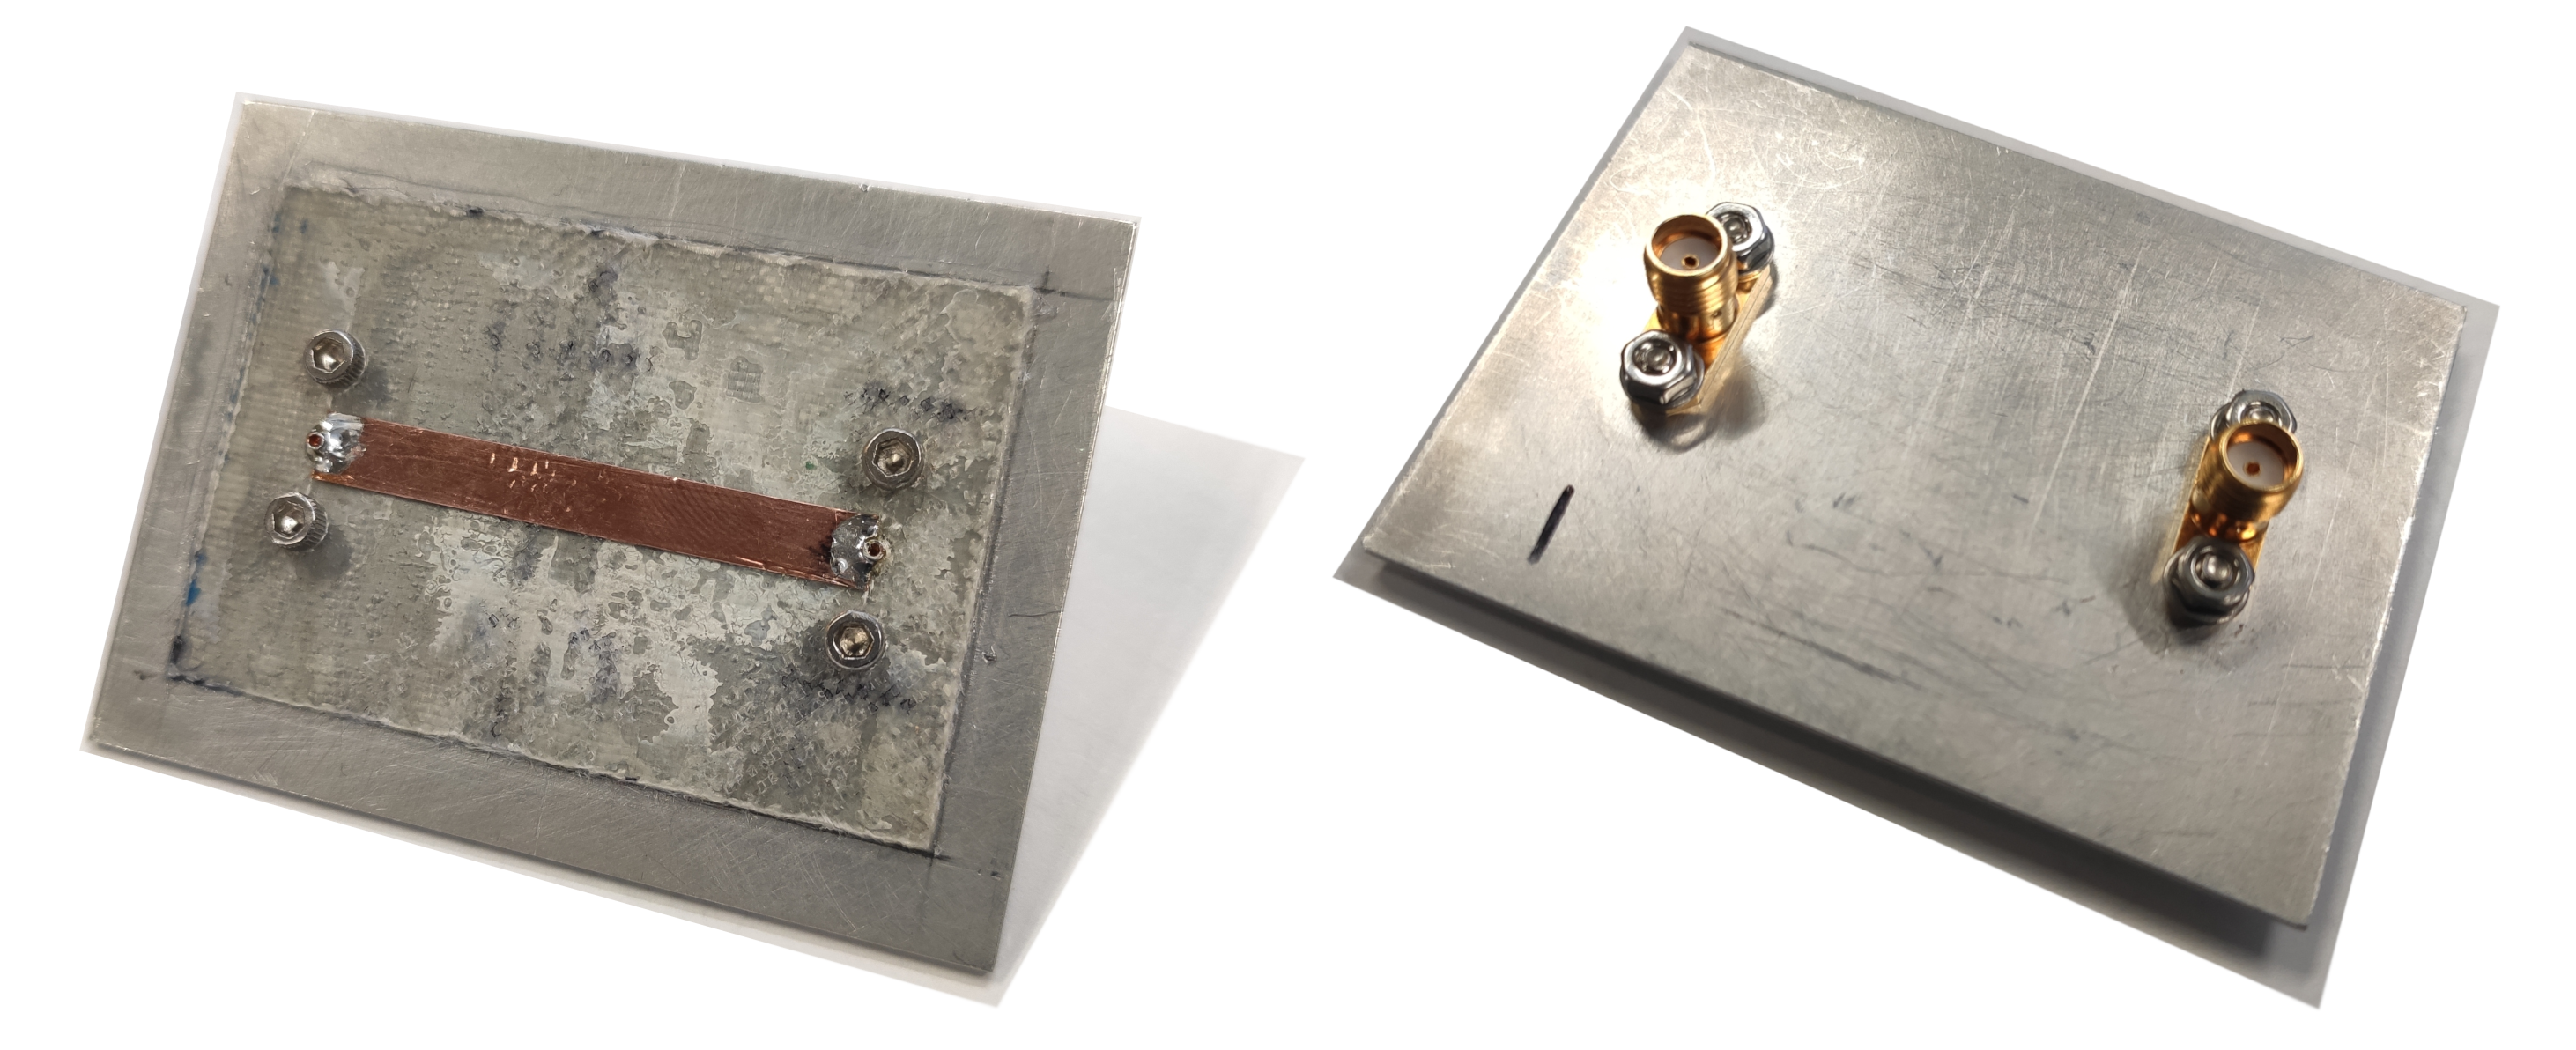
\includegraphics[width=\textwidth]{fixture}
        \caption{Shortest (40~mm) line test fixture. Front: 5~mm~x~40~mm adhesive copper trace on glass fiber panel.
        Back: thru-hole SMA connector with m2.5 screws and bolts.}
        \label{fig:photo}
    \end{figure}
    This report contains the results for the microstrip line test produced using vector measurements of the reflection
    and transmission frequency response of three test fixtures of different lengths.
    The shorter fixture is shown in \fig{fig:photo}.
    The three fixtures feature a microstrip line built using an adhesive copper strip 5~mm wide on a piece of dielectric
    composite (Material Under Test) glued on a supporting aluminium slab.
    Two thru-hole connectors are bolted to the structure with the central pin trimmed to length and soldered to the copper line.
    From here on, the fixtures are referred to by their line length; respectively: long~=~219~mm (L), medimum~=~146~mm (M), and
    short~=~40mm (S).\\
    The complex propagation coefficient $\gamma$ extraction procedure is defined in \ref{doc:microstrip-characterization} and
    applied here with minor modifications.
    An overview of the methodology and the results of this de-embedding procedure are reported in~\sref{sec:de-embedding}.\\
    The error sensitivity to small differences in the average permittivity of the fixtures is derived in~\sref{sec:error}
    in an effort to explain the discrepancies found in the results of~\sref{sec:de-embedding}.\\
    The procedure for fitting the measured datum to a CST microstrip model is reported in~\sref{sec:numerical-model-matching}
    along with the resulting permittivity and loss tangent of the \emph{Material Under Test} (MUT).\\
    The conclusions are drawn in~\sref{sec:conclusion}.


    \section{Fixtures assembly and geometrical variability}
    \label{sec:assembly}


    \section{De-embedding results}
    \label{sec:de-embedding}

    %% De embedding procedure modification

    %% results outline

    The de-embedding results (virtual transmission line properties) are here presented in terms of:
    \begin{itemize}
        \item Transmissivity, i.e., the S21 of the de embedded length of transmission line, denoted with \emph{t}.
        \item Reflectivity, i.e., the S21 of the de embedded length of transmission line, denoted with \emph{s}.
        \item Effective permittivity $\varepsilon_{eff}$.
        \item Effective loss tangent $\tan\delta_{eff}$.
    \end{itemize}
    The effective permittivity and loss tangent are for visualization purposes only and are formulated from the low-loss
    approximation~\cite{Pozar} for transmission lines (assuming all loss lumped into the dielectric material and
    the phase velocity independent of loss).\\
    The effective permittivity is given by
    \begin{equation}
        \varepsilon_{eff} = \left(\dfrac{ c [\text{unwrap}(\angle{t}) + n2\pi]} {2\pi f L}\right)^2,
        \label{eq:epsilon}
    \end{equation}
    where $c$ is the speed of light, $L$ is the line length (length difference between the two fixtures),
    $f$ is the frequency and $n$ an integer to correctly reconstruct the true--time phase delay
    (usually n=0 if the first sample of $f$ is small enough).\\
    The loss tangent is defined as
    \begin{equation}
        \tan \delta_{eff} = -\dfrac{\ln(|t|) c}{L \pi f \sqrt{\varepsilon_{eff}}}.
        \label{eq:tand}
    \end{equation}
    A better figure that can be used to make the measurement results independent from the physical length $L$, is the
    complex propagation constant
    \begin{equation}
        \gamma = \alpha + j \beta = \ln(t) / L,
        \label{eq:gamma}
    \end{equation}
    used in \sref{sec:numerical-model-matching} to match the CST model to the measured data.\\

    Note how all the above depend (measurand) exclusively on the transmissivity $t$.
    While, the reflectivity $s$, using the de-embedding procedure of~\ref{doc:microstrip-characterization}, can be
    considered as a function of the de-embedding error, as it should be 0 in the ideal case. \\
    For the measured data, it was noted that the response $s$ varies changing the gate width from the, originally considered, distance between
    two reflections to a smaller value.
    Since this changes improves or degrades the value of $s$ in different parts of the spectrum, it was chosen to modify
    the de-embedding algorithm of~\ref{doc:microstrip-characterization}, to sweep over several values for the gate width
    and then perform a weighted average of the different resulting $t$--curves using the $s$--curves as a logarithmic
    weighting factors for every frequency bin .\\
    This sensibility to changes in the gates widths is probably due to some irregularities in the measured transmission lines,
    far from being perfectly homogeneous due to the manufacturing process.
    This change in gate length, in theory, should not impact negatively on the overall result as it is equivalent to
    performing a low-pass filtering of the time impulse response of the transitions to be removed.
    In fact, the average $s$ value over frequency reduces when this weighted average technique is introduced. \\
    Moreover, instead of always using the longer transmission line to generate the transition scattering matrices to de--embedd the
    shorter transmission line, all combinations of measurement/simulation pairs are computed.
    Although using the longer line as reference provides the best theoretical frequency resolution, is interesting to see
    what happens in the reversed case where the transition scattering parameters have a naturally shorter (low--pass)
    time response, and hence a smoother shape in frequency.\\
    The resulting de-embedded virtual lines can therefore either have a causal or an anti--causal response.
    For ease of comparison all the signs in the data plots are normalized to always represent the equivalent anti--causal
    transmission lines, e.g., \laser{LS} is the \emph{anti-causal} (negative length) line obtained de--embedding the line S from the transitions
    T-matrices obtained from the response of L, and vice versa \laser{SL} is the \emph{causal} line of identical positive length.

    \subsection{Simulated data baseline}
    \label{subsec:simulation}
    \begin{figure}[!t]
        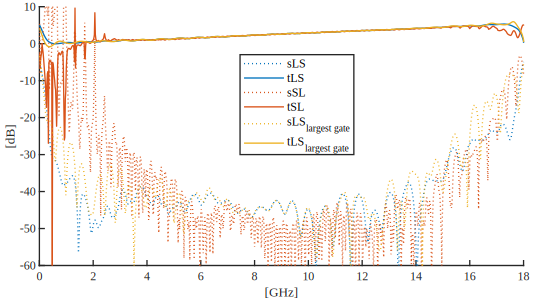
\includegraphics[width=\textwidth]{sparasim}
        \caption{De-embedding results from full wave simulations of a 40~mm (S) and a 219~mm (L) test fixtures.
        Solid lines: transmissivity (s), dotted lines: reflectivity (t); for all the combinations plus LS deembedding
        without gate width variation. The transmissivity sign is chosen to always correspond to a negative-length section
        of lossy transmission line (for ease of comparison).}
        \label{fig:sparasim}
    \end{figure}
    \begin{figure}[!tb]
        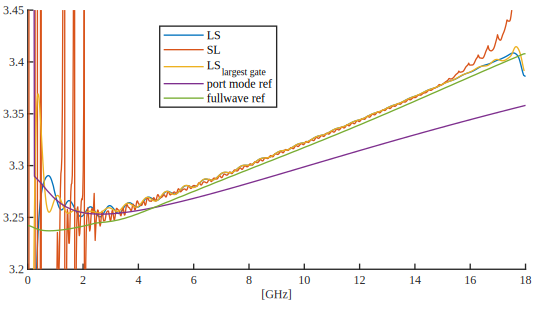
\includegraphics[width=\textwidth]{epsisim}
        \caption{Simulated data retrieved effective permittivity compared with $\varepsilon_{eff}$ calculated from
        the $S_{21}$ of a full--wave simulation of a microstrip section (terminated on adaptive waveguide ports),
            and effective dielectric constant computed by the port mode solver of CST.}
        \label{fig:epsilonsim}
    \end{figure}
    \begin{figure}[!tb]
        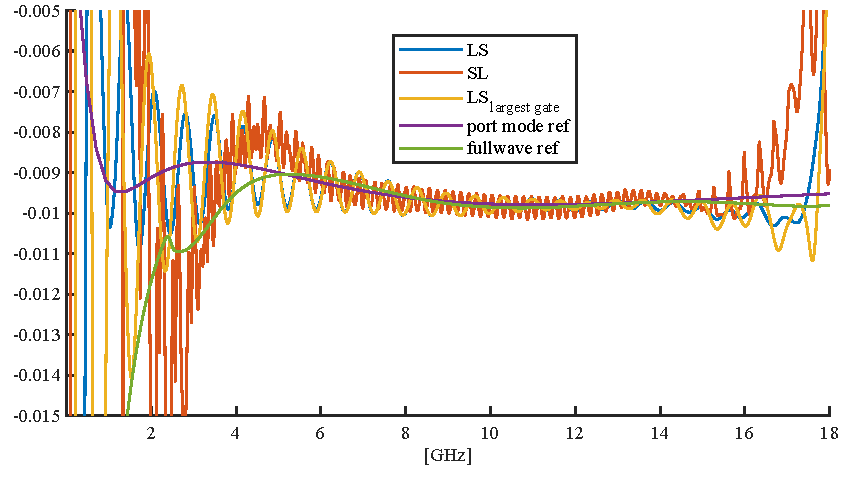
\includegraphics[width=\textwidth]{tandsim}
        \caption{Simulated data retrieved effective loss tangent compared with $\tan\delta_{eff}$ calculated from
        the $S_{21}$ of a full--wave simulation of a microstrip section (terminated on adaptive waveguide ports),
            and effective loss tangent computed by the port mode solver of CST.}
        \label{fig:tandsim}
    \end{figure}
    In order to validate the modified de-embedding algorithm, a run wit simulated data, from the same CST models
    of~\ref{doc:microstrip-characterization} was performed.
    To observe the effect of the weighted average step, one run for the de-embedding algorithm is set to use the widest
    possible gate (as in~\ref{doc:microstrip-characterization}).
    The S-parameter results in~\fig{fig:sparasim} show that the averaging slightly improves on the ripple and the $s$
    response (especially at the edges) wile not changing substantially the response.
    The permittivity,~\fig{fig:epsilonsim}, and loss tangent~\fig{fig:tandsim}, results are compared with the
    equivalent values computed form the complex propagation constant of the waveguide port mode solver of CST, and
    from a full-wave simulation of a section of microstrip line terminated on to two adaptive waveguide ports.\\
    The reason behind the large difference between the port mode solver result and and the full wave solution in~\fig{fig:epsilonsim}
    is unclear.
    The slight difference between the de-embedding results and the full wave result (in~\fig{fig:epsilonsim}), instead,
    might be caused by a phase error due to finite meshing of the model or other numerical inaccuracies.
    The full-wave reference should be in any case the most accurate representation of the de-embedded virtual line and the
    total error appears reasonably small.\\
    The results in~\fig{fig:tandsim} seem all to be in good agreement (at least in the central portion of the spectrum),
    with ripple and \emph{edge diffraction} effects that seem to be most severe in the \laser{SL} case.

    \subsection{Measurements}
    \label{subsec:measurements}
    \begin{figure}[!tb]
        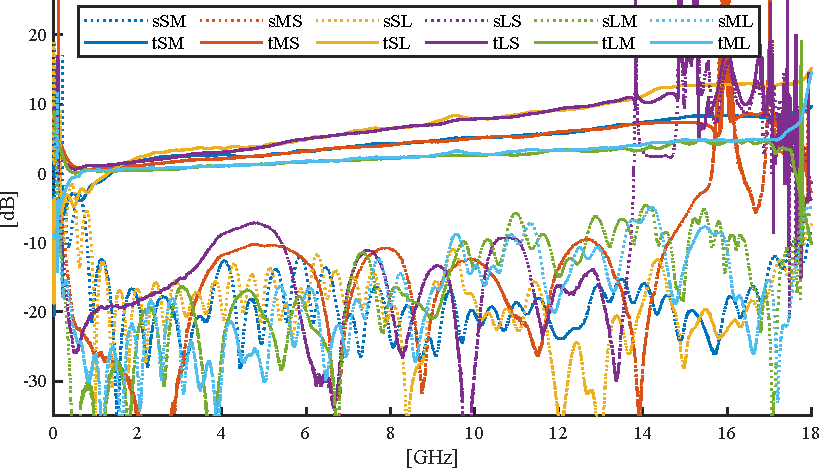
\includegraphics[width=\textwidth]{sparameas}
        \caption{De-embedding results from the measurements of the test fixtures.
        Solid lines: transmissivity (s), dotted lines: reflectivity (t);
        for all the reference-fixture -- under-test-fixture combinations e.g. LS = long line as reference and short line de-embedding target.
        The transmissivity sign is chosen to always correspond to a negative-length section
        of lossy transmission line (for ease of comparison).}
        \label{fig:sparameas}
    \end{figure}
    \begin{figure}[!tb]
        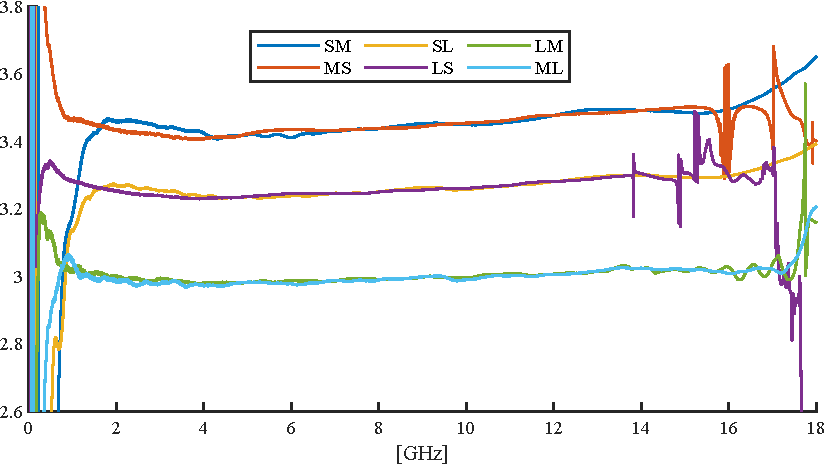
\includegraphics[width=\textwidth]{epsimeas}
        \caption{Measured data retrieved effective permittivity for all the reference-fixture -- under-test-fixture combinations.}
        \label{fig:epsilonmeas}
    \end{figure}
    \begin{figure}[!tb]
        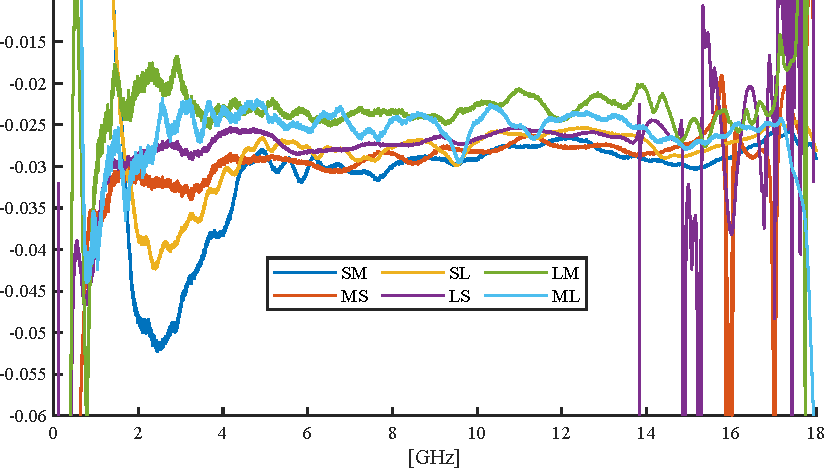
\includegraphics[width=\textwidth]{tandmeas}
        \caption{Measured data retrieved effective loss tangent for all the reference-fixture -- under-test-fixture combinations.}
        \label{fig:tandmeas}
    \end{figure}

    The measurements are made connecting the test fixtures to the PNA with two APC7 to APC3.5 adapters.
    The instrument is calibrated at the APC7 interface, there is no need to calibrate the 3.5 connectors as they can be
    considered as part of the transition to be removed during the de-embedding by performing two measurements for every
    fixture as described here.\\
    For every fixture, two measurements are taken.
    The first with the port 1 of the PNA connected to the port 1 of the fixture (e.g., marked in~\fig{fig:photo}) and
    port 2 of the PNA to the port 2 of the fixture.
    In the second measurement, the fixture is rotated to connect the port 1 of the PNA to the port 2 of the fixture and
    vice-versa.
    Averaging all the S-parameters of the two measurements imposes a virtual symmetry condition that effectively removes
    all differences in the right and left connector adapters for all fixtures alike.
    An additional averaging is performed before the de--embedding to remove the asymmetries inside each individual test
    fixture otherwise presenting different S11 and S22.
    The transmissivity and reflectivity of every fixture for the purpose of de-embedding are then defined as
    \begin{equation}
        S11 = \dfrac{1}{4}(S11_a + S11_b + S22_a + S22_b),
        \label{eq:saverage}
    \end{equation}
    and
    \begin{equation}
        S21 = \dfrac{1}{4}(S21_a + S21_b + S12_a + S12_b),
        \label{eq:taverage}
    \end{equation}
    where the subscripts $a$ and $b$ denote the two PNA measurements made for every fixture.\\
    The de-embedded transmissivity and reflectivity are displayed in~\fig{fig:sparameas}.
    The residual reflection $s$ is higher than for the simulated case, but still acceptable especially in X-band (8--12~GHz).
    Inverting the reference and de-embedded fixture seems to only have a minor effect on the responses.\\
    The effective permittivity in~\fig{fig:epsilonmeas} (derived from the phase component of $t$) is the one showing
    the largest deviation between pairs of test fixtures.
    This is probably due to a difference in the permittivity of the two fixtures used in the de--embedding, the error
    is also amplified in the case of a shorter difference length, as motivated in the next section.
    Using the results of~\sref{sec:error} the \laser{LS--SL} and \laser{MS--SM} results are the ones which should better
    approximate the effective permittivities of the longest of the two lines used in the de--embedding procedure, i.e.
    \laser{L} and \laser{M} respectively.\\
    The loss tangent in~\fig{fig:tandmeas} also shows some differences, with the measurements \laser{LM--ML} more distant
    than the other two pairs.
    Recall, in fact, that the tangent delta is computed from the square root of the dielectric constant~\eqref{eq:tand}
    and therefore the error will be propagated from one to another.


    \section{Non-identical fixtures de-embedding error}
    \label{sec:error}
    \begin{figure}[!b]
        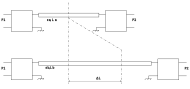
\includegraphics[width=\textwidth]{error}
        \caption{Two--fixtures schematic for the de-embedding procedure. The transitions are identical and the lines are
        of different lengths to produce a $\Delta_L$--long virtual line response. The error arises from the difference
        in phase velocity between the two lines (related to the effective permittivities $\varepsilon$).}
        \label{fig:error}
    \end{figure}
    In the ideal case, the two test fixtures are supposed to have identical propagation constants.
    In practice, as depicted in~\fig{fig:error}, the two lines might have slightly different properties, yielding
    to an error in the estimation of the electrical length of the virtual line $\Delta_L$ in the drawing.\\
    Assuming that the only difference is in the phase velocity of the two lines (and any impedance mismatch between the
    two lines is negligible), the de-embedding procedures will still be removing the effect of transitions, but also a
    length of transmission line proportional to $\sqrt{\varepsilon_a }L_a$ (the shortest of the two).
    The resulting electrical length $\Delta_L$, however, will not be the physical length difference of the two lines
    but something proportional to the phase delays difference $\propto (\sqrt{\varepsilon_b} L_b - \sqrt{\varepsilon_a} L_a$).
    This setup leads to the following estimation for the dielectric constant~\eqref{eq:epsilon} (e.g.,~\fig{fig:epsilonmeas})
    \begin{equation}
        \sqrt{\varepsilon} = \dfrac{L_b \sqrt{\varepsilon_b} - L_a \sqrt{\varepsilon_a}}{L_b - L_a}
        \label{eq:epsidiff}
    \end{equation}
    which would not depend on $L_b$ and $L_a$ if $\varepsilon_a = \varepsilon_b$.\\
    Assuming we are interested in finding $\varepsilon_b$, and there is a permittivity error $\Delta\varepsilon$ between
    the two fixtures such as $\varepsilon_a = \varepsilon_b+\Delta\varepsilon$, the de-embedding result $\varepsilon$
    will deviate from the desired $\varepsilon_b$ of a quantity
    \begin{equation}
        \varepsilon_{err} = \varepsilon_b -
        \left(\dfrac{L_b \sqrt{\varepsilon_b} - L_a \sqrt{\varepsilon_b+\Delta\varepsilon}}{L_b - L_a}\right)^2.
        \label{eq:epsierror}
    \end{equation}
    The error in~\eqref{eq:epsierror}, will be null in the case $\Delta\varepsilon = 0$, in the general case we can
    study its sensitivity to $\Delta\varepsilon$ variations
    \begin{equation}
        \dfrac{\partial \varepsilon_{err}}{\partial \Delta\varepsilon} =
        - \dfrac{L_a^2}{(L_b - L_a)^2} +
        \dfrac{L_b L_a}{(L_b - L_a)^2} \dfrac{\varepsilon_b}{\sqrt{\varepsilon_b(\varepsilon_b + \Delta\varepsilon)}},
        \label{eq:errderivative}
    \end{equation}
    which can be further simplified in the case of $\Delta\varepsilon \rightarrow 0$ (small perturbations)
    \begin{equation}
        \left.\dfrac{\partial \varepsilon_{err}}{\partial \Delta\varepsilon}\right|_{\Delta\varepsilon = 0}=
        - \dfrac{L_a^2}{(L_b - L_a)^2} +
        \dfrac{L_b L_a}{(L_b - L_a)^2},
        \label{eq:smallerr}
    \end{equation}
    exclusively dependent on the line lengths. \\
    The result in~\eqref{eq:smallerr} tells us that a small error in the phase velocity of two fixtures, will be
    amplified by the de-embedding algorithm, if $L_b - L_a$ is too small.
    Furthermore, since~\eqref{eq:epsierror}\eqref{eq:errderivative}\eqref{eq:smallerr} all assume $L_b > L_a$,the error
    from~\eqref{eq:smallerr} will always be positive for small $\Delta\varepsilon$, meaning that $\varepsilon$~\eqref{eq:epsidiff}
    will allways be smaller than the measurand $\varepsilon_b$.

    \subsection{Measurement results}
    \label{subsec:measure-error}
    \begin{table}[!ht]
        \centering
        \begin{tabular}{|l|l|l|l|l}
            \cline{1-4}
            $L_b$ {[}mm{]} & $L_a$ {[}mm{]} & $\Delta_L$ {[}mm{]} & $\dfrac{\partial \varepsilon_{err}}{\partial \Delta\varepsilon}$  \rule[-4mm]{0mm}{11mm}&  \\ \cline{1-4}
            219            & 40             & 179                 & 0.22                                                                                   & \\ \cline{1-4}
            219            & 146            & 73                  & 2.0                                                                                    & \\ \cline{1-4}
            146            & 40             & 106                 & 0.37                                                                                   & \\ \cline{1-4}
        \end{tabular}
        \caption{Measurement sensitivity to permittivity variations.}
        \label{tab:errorsensitivity}
    \end{table}
    Tabulating~\eqref{eq:smallerr} for the 3 test fixture combinations we obtain~\ref{tab:errorsensitivity}.
    These values explain the difference in the results in~\fig{fig:epsilonmeas} (and consequently~\fig{fig:tandmeas}).
    Also we can say that the measurements \laser{LS--SL} are the ones that best approximate the characteristics of the
    longest line \laser{L} (due to the smaller error sensitivity), while the measurements \laser{LM--ML} are the worst
    in this case.\\
    By extension, assuming that \laser{LS--SL} and \laser{MS--SM} are good approximations for the properties of
    \laser{L} and \laser{M} respectively, we still find a difference of $\approx$~0.265 in the effective dielectric
    permittivity indicating a substantial difference between test fixtures.\\
    The dielectric thickness differences measured during the assembly process might be part of the reason for this error.
    However, varying the thickness of the material in a CST model, doesn't produce a change in $\varepsilon_{eff}$
    large enough to justify the error.
    Therefore the reason must lie in some non-homogeneity of the material due to manufacturing errors.
    In this sense, the measurement \laser{LS--SL} should represent a better \emph{average} of non-idealities effects;
    and will be used to match a numerical model to the measurement.


    \section{Numerical model matching}
    \label{sec:numerical-model-matching}
    \begin{figure}[!b]
        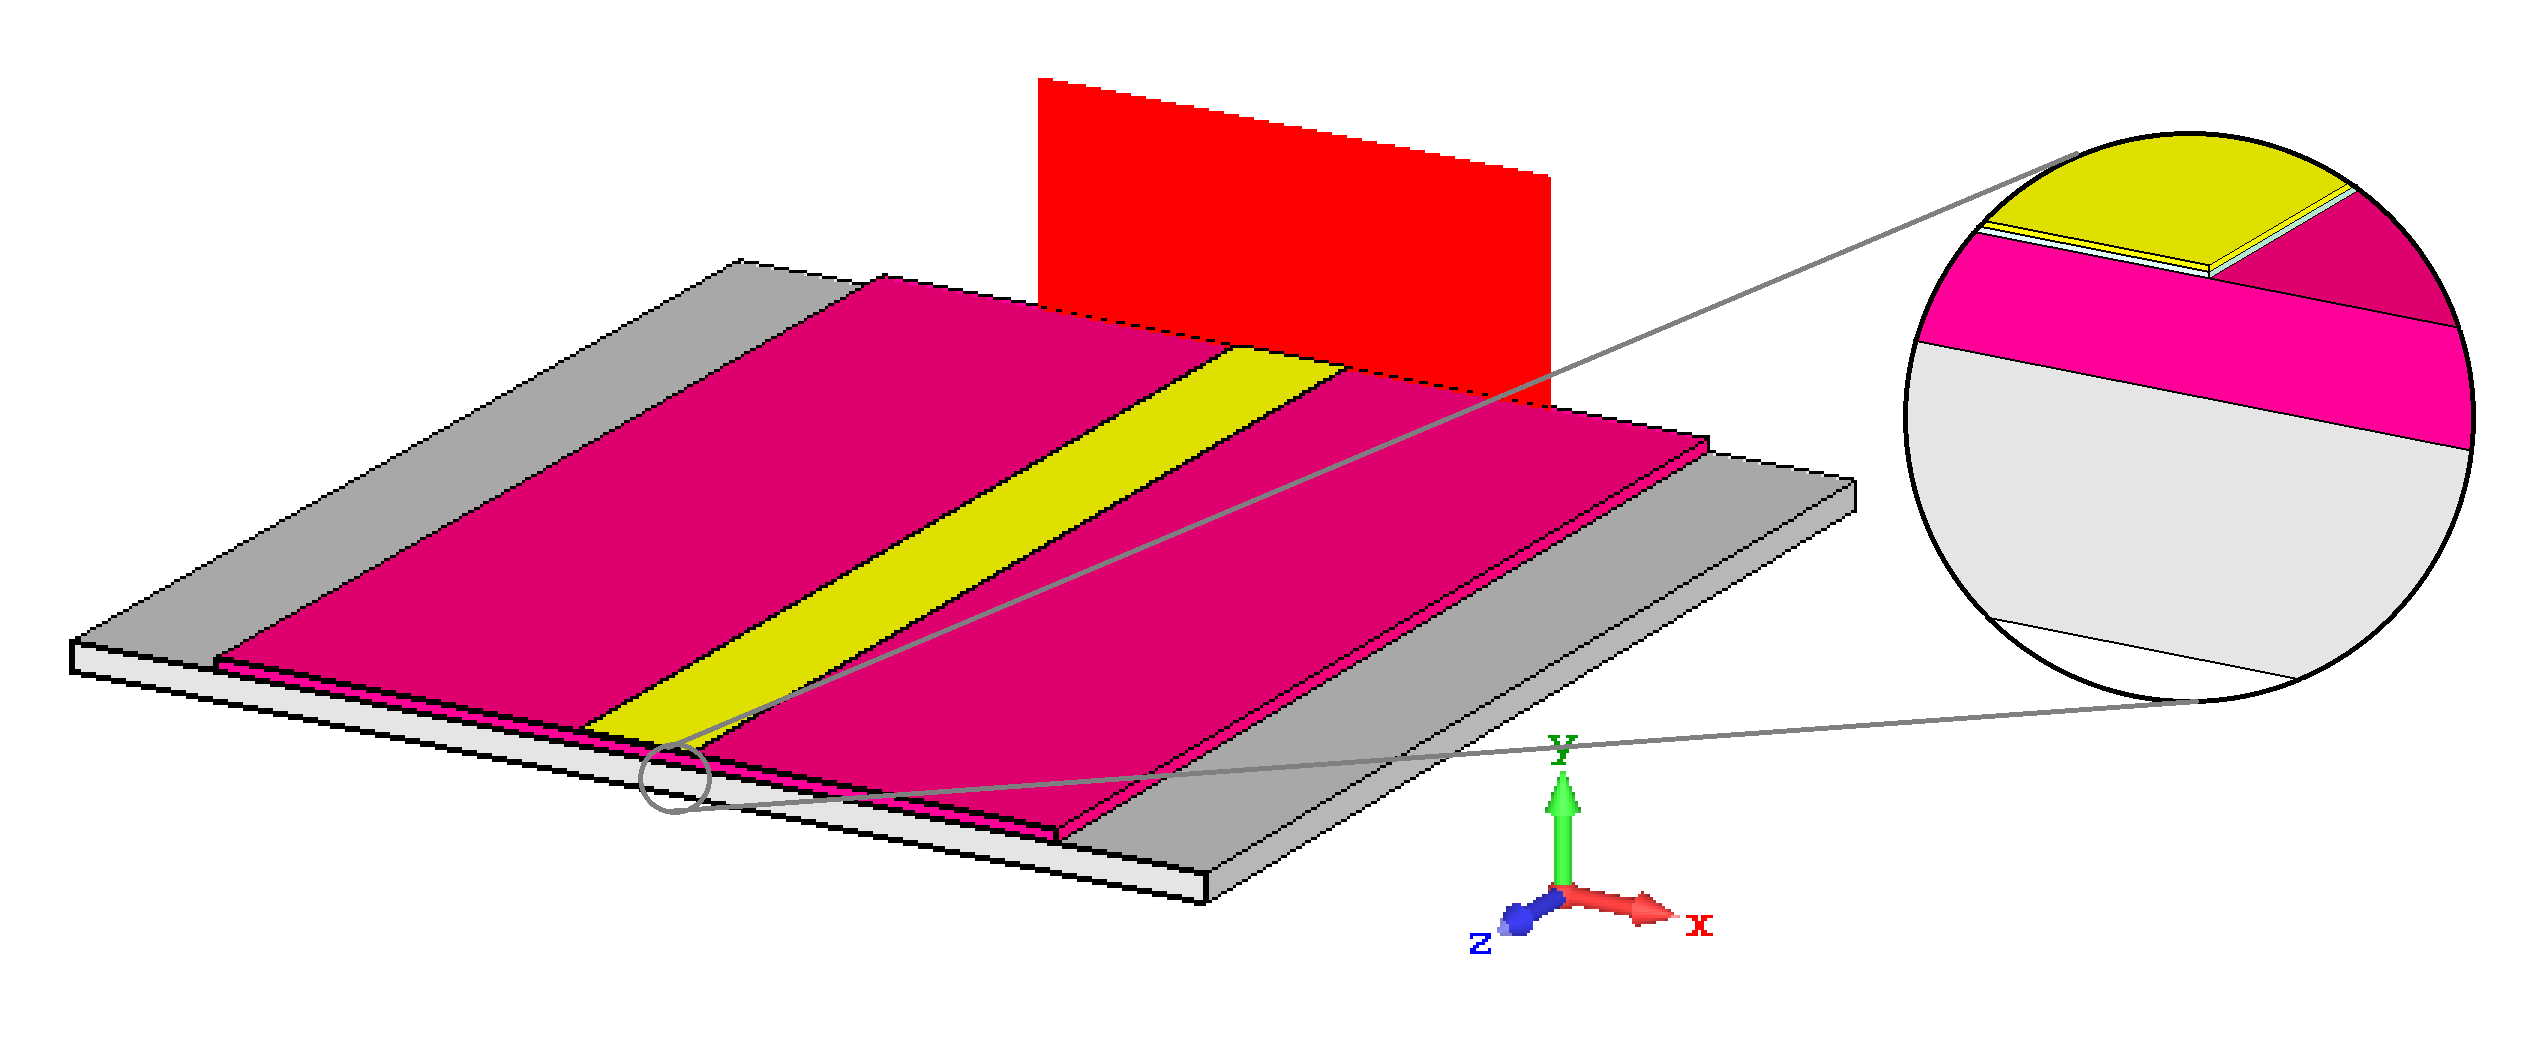
\includegraphics[width=\textwidth]{fitter}
        \caption{CST model for the microstrip, the layers from top to bottom are: copper 0.3~mm, acrylic 0.3~mm
            (adhesive), MUT 0.55~mm, aluminium 1.2~mm.}
        \label{fig:fitter}
    \end{figure}
    The $LS$ measure was fitted to the model in~\fig{fig:fitter} using the difference of $\gamma$~\eqref{eq:gamma}
    as a frequency-dependent error function.
    This error curve is integrated over a specified portion of the bandwidth to produce an error value that can be used
    in a optimizer.\\
    The optimization is performed with a python script that controls the execution of CST and updates the values of the
    dielectric constant and loss tangent of the MUT between iterations.\\
    The \laser{minimize} function of the library \laser{scipy} is used for the optimization.
    Different methods can be utilized, the quasi-Newton \emph{BCGF} and the \emph{Nelder-Mead} methods where both found
    effective (the latter is best if the initial solution is far from convergence).


    %    \subsection{Sensitivity considerations}
    %    \label{subsec:sensitivity}


    \section{Conclusions}
    \label{sec:conclusion}
    The manufacturing process needs to be improved for repeatability.
    The material is lossy, might still be usable for a reflectarray, definitely not a good choice for traveling--wave antennas.

    \clearpage
    \bibliographystyle{IEEEtran}
    \bibliography{bibliography}

\end{document}

